%% %% %% %%
%%
%% Previo de la práctica
%% [No hubo previo]
%%
%% %% %% %%

\documentclass[../procedimientos.tex]{subfiles}
\graphicspath{{\subfix{../../images/}}}

\begin{document}
\subsection{Previo} \label{subs:previo}
\subsubsection*{Pregunta 1}
\begin{em}
  Un circuito desplazador-rotador de 4 bits es un módulo combinacional que 
  tiene como entrada una palabra de 4 bits $X=X_3X_2X_1X_0$, una palabra 
  $Z=Z_3Z_2Z_1Z_0$ de 4 bits como salida, y tres entradas de control: $s$, $d$  
  y $r$, que actúan como se indica a continuación.

  Si $s=0$, la salida refleja la entrada. Si $s=1$, entonces la entrada es 
  desplazada en 1 bit en la dirección indicada por $d$. Si $d=0$ y $s=1$, 
  entonces el circuito desplaza la entrada 1 bit a la derecha.  Si $d=1$ y 
  $s=1$, la entrada es desplazada a la izquierda. El bit $r$ indica si el 
  circuito actúa como desplazador o como rotador. Es decir, si $sdr=100$, la 
  salida corresponde a la entrada desplazada a la derecha, y el nuevo bit 
  $Z_3=0$. En cambio, si $sdr=101$, el nuevo bit $Z_3$ corresponde al bit 
  $X_0$.  Asimismo, si $sdr=110$, la salida corresponde a la entrada 
  desplazada a la izquierda, y el nuevo bit $Z_0$ es $0$. En cambio, si 
  $sdr=111$, el nuevo bit $Z_0$ corresponde al bit $X_3$.

  Diseñe este circuito usando \textbf{sólo multiplexores de 4 entradas}.  
  Utilice tantos como encuentre necesario.
\end{em}

Podemos ver que este problema se trata de un problema de selección de bits, 
por lo cual es posible llevarlo a cabo hacienod uso únicamente de 
multiplexores. Existen diversas aproximaciones, pero la más eficiente que se 
encontró fue la siguiente. Para cada bit $z_n$ de salida, se tiene que existen 
los siguientes casos en función de los bits de entrada $x_n$:
\begin{table}[H]
  \centering
  \begin{tabular}{ccc|cccc}
    $s$ & $d$ & $r$ & $z_3$ & $z_2$ & $z_1$ & $z_0$\\
    \hline
    0 & 0 & 0 & $x_3$ & $x_2$ & $x_1$ & $x_0$\\
    0 & 0 & 1 & $x_3$ & $x_2$ & $x_1$ & $x_0$\\
    0 & 1 & 0 & $x_3$ & $x_2$ & $x_1$ & $x_0$\\
    0 & 1 & 1 & $x_3$ & $x_2$ & $x_1$ & $x_0$\\
    1 & 0 & 0 & 0     & $x_3$ & $x_2$ & $x_1$\\
    1 & 0 & 1 & $x_0$ & $x_3$ & $x_2$ & $x_1$\\
    1 & 1 & 0 & $x_2$ & $x_1$ & $x_0$ & 0    \\
    1 & 1 & 1 & $x_2$ & $x_1$ & $x_0$ & $x_3$
  \end{tabular}
\end{table}

Los casos que devuelven $0$ se encuentran en los extremos ya que únicamente 
son los únicos que tienen modificaciones con respecto al bit $r$. Casi todas 
las salidas se definen en función de $s$ y $d$; a excepción de los casos que 
devuelven $0$ directamente.

Primero, se crean utilizan dos multiplexores que se cierta forma trabajan de 
forma auxiliar. Se basan en los valores de entrada $d$ y $r$.
\begin{itemize}
  \item Para el primer caso, lo que se requiere es que devuelva $0$ cuando 
    $dr=10$, de lo contrario, que devuelva el valor $x_3$. Con esto, se 
    selecciona el bit que irá hasta la izquierda dependiendo si se trata de 
    una rotación o un desplazamiento. La salida se puede llamar $k_0$.
    \begin{itemize}
      \item $00 \rightarrow x_3$
      \item $01 \rightarrow x_3$
      \item $10 \rightarrow 0$
      \item $11 \rightarrow x_3$
    \end{itemize}
  \item Para el segundo caso, lo que se requiere es que devuelva $0$ cuando 
    $dr=00$, de lo contrario, que devuelva el valor $x_0$. Con esto, se 
    selecciona el bit que irá hasta la izquierda dependiendo si se trata de 
    una rotación o un desplazamiento. La salida se puede llamar $k_3$.
    \begin{itemize}
      \item $00 \rightarrow 0$
      \item $01 \rightarrow x_0$
      \item $10 \rightarrow x_0$
      \item $11 \rightarrow x_0$
    \end{itemize}
\end{itemize}

Lo anterior debe ser combinado con un comportamiento adicional para que pueda 
funcionar de forma adecuada. $k_0$ es el bit correspondiente a $z_0$ en caso 
de que se tenga $sd=11$, mientras que $k_3$ es el bit correspondiente a $z_3$ 
en caso de que se tenga $sd=10$. Hace falta tomar en cuenta las demás 
combinaciones, pero es posible simplificar un poco la tabla anterior con ayuda 
de los valores auxiliares ($k_0$ y $k_3$) que calculamos previamente.
\begin{table}[H]
  \centering
  \begin{tabular}{ccc|cccc}
    $s$ & $d$ & $r$ & $z_3$ & $z_2$ & $z_1$ & $z_0$\\
    \hline
    0 & 0 & 0 & $x_3$ & $x_2$ & $x_1$ & $x_0$\\
    0 & 0 & 1 & $x_3$ & $x_2$ & $x_1$ & $x_0$\\
    0 & 1 & 0 & $x_3$ & $x_2$ & $x_1$ & $x_0$\\
    0 & 1 & 1 & $x_3$ & $x_2$ & $x_1$ & $x_0$\\
    1 & 0 & 0 & $k_3$ & $x_3$ & $x_2$ & $x_1$\\
    1 & 0 & 1 & $k_3$ & $x_3$ & $x_2$ & $x_1$\\
    1 & 1 & 0 & $x_2$ & $x_1$ & $x_0$ & $k_0$\\
    1 & 1 & 1 & $x_2$ & $x_1$ & $x_0$ & $k_0$
  \end{tabular}
\end{table}

Lo siguiente es similar para todos los términos. Dependiendo del valor de los 
bits $s$ y $d$, se selecciona el bit indicado por la tabla anterior. Se tienen 
entonces otros cuatro multiplexores.
\begin{itemize}
  \item Para el caso de $z_0$, se tiene que:
    \begin{itemize}
      \item $00 \rightarrow x_0$
      \item $01 \rightarrow x_0$
      \item $10 \rightarrow x_1$
      \item $11 \rightarrow k_0$
    \end{itemize}
  \item Para el caso de $z_1$, se tiene que:
    \begin{itemize}
      \item $00 \rightarrow x_1$
      \item $01 \rightarrow x_1$
      \item $10 \rightarrow x_2$
      \item $11 \rightarrow x_0$
    \end{itemize}
  \item Para el caso de $z_2$, se tiene que:
    \begin{itemize}
      \item $00 \rightarrow x_2$
      \item $01 \rightarrow x_2$
      \item $10 \rightarrow x_3$
      \item $11 \rightarrow x_1$
    \end{itemize}
  \item Para el caso de $z_3$, se tiene que:
    \begin{itemize}
      \item $00 \rightarrow x_3$
      \item $01 \rightarrow x_3$
      \item $10 \rightarrow k_3$
      \item $11 \rightarrow x_2$
    \end{itemize}
\end{itemize}

Combinando los comportamientos anteriores se obtiene el circuito deseado, tal 
como se muestra en la Figura \ref{fig:previo1}. En donde en total se hizo uso 
de \textbf{seis multiplexores}.
\begin{figure}[H]
  \centering
  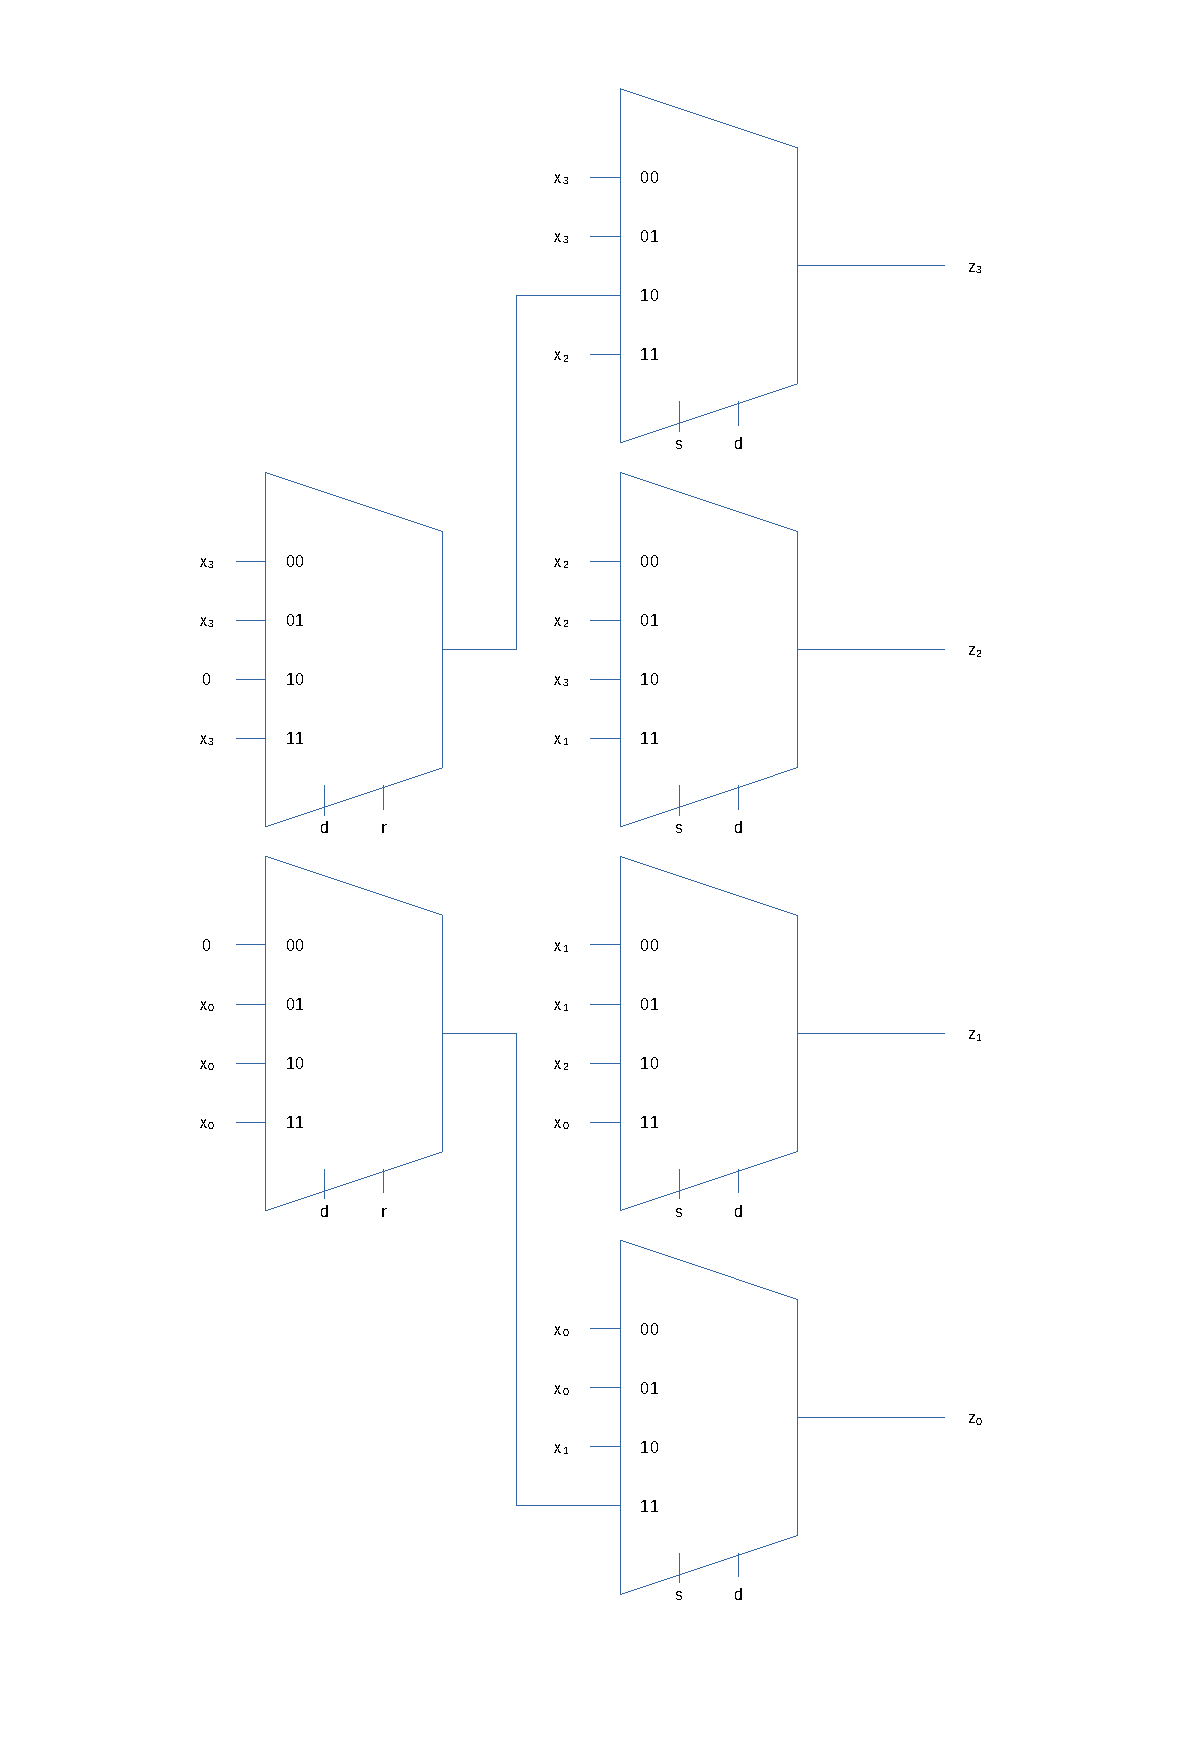
\includegraphics[width=0.6\textwidth]{previo-1}
  \caption{Circuito desplazador-rotador (Previo)}
  \label{fig:previo1}
\end{figure}

\subsubsection*{Pregunta 2}
\begin{em}
  Construir un convertidor a siete segmentos de su respectivo número de cuenta
\end{em}

\end{document}

